%%%%% Design %%%%%
\chapter{The Code Display}
\label{append:code_display}
\begin{figure}[H] %[H] "corresponds to start the figure Here" 
    \centering %alignment can be flushleft or flushright
    \captionsetup{labelsep=colon}
    \begin{subfigure}{\textwidth} % subfigure 2
        \centering
        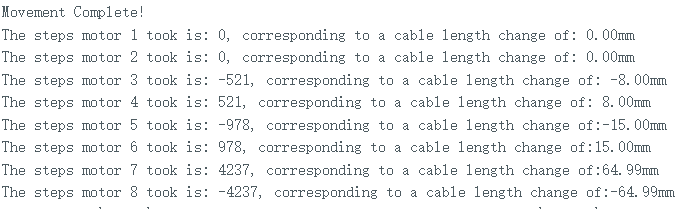
\includegraphics[width=\linewidth]{Image/Code-Display/arduino2.png}
        \caption{\centering the result of first stepping test}
        \label{fig:arduino_code_display_2}
    \end{subfigure}
    \begin{subfigure}{\textwidth} % subfigure 3
        \centering
        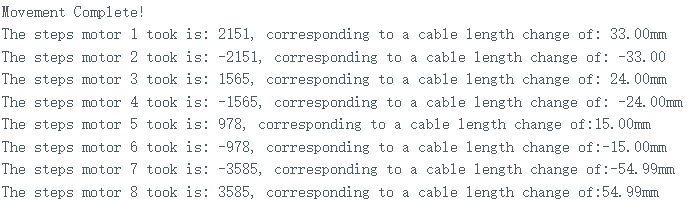
\includegraphics[width=\linewidth]{Image/Code-Display/arduino3.png}
        \caption{\centering the result of second stepping test}
        \label{fig:arduino_code_display_3}
    \end{subfigure}
    \caption[The Display of Arduino Control System]
    {\centering \textbf{The Display of Arduino Control System.}}
    \label{fig:arduino_code_display}
\end{figure}

\begin{figure}[H] %[H] "corresponds to start the figure Here" 
    \centering %alignment can be flushleft or flushright
    \captionsetup{labelsep=colon}
    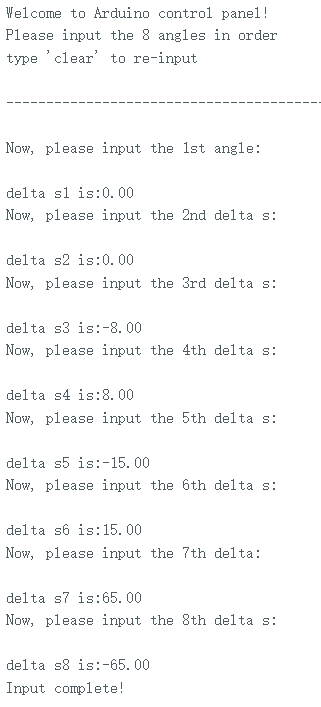
\includegraphics[width=0.65\linewidth]{Image/Code-Display/arduino1.png}
    \caption[The input parameters for first stepping test]
    {\centering \textbf{The input parameters for first stepping test.}}
    \label{fig:arduino_code_display_1}
\end{figure}

\begin{figure}[H] %[H] "corresponds to start the figure Here" 
    \centering %alignment can be flushleft or flushright
    \captionsetup{labelsep=colon}
    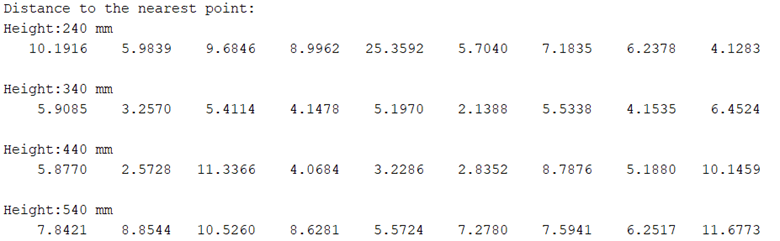
\includegraphics[width=0.65\linewidth]{Image/Code-Display/matlab_240.png}
    \caption[The detection result while index=1000000 and H=240]
    {\centering \textbf{The detection result while index=1000000 and H=240.}}
    \label{fig:matlab_240}
\end{figure}
\begin{figure}[H] %[H] "corresponds to start the figure Here" 
    \centering %alignment can be flushleft or flushright
    \captionsetup{labelsep=colon}
    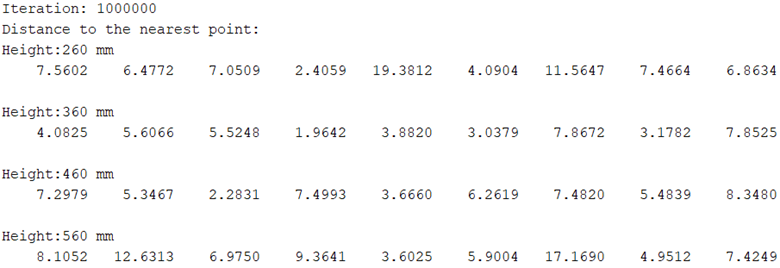
\includegraphics[width=0.65\linewidth]{Image/Code-Display/matlab_260.png}
    \caption[The detection result while index=1000000 and H=260]
    {\centering \textbf{The detection result while index=1000000 and H=260.}}
    \label{fig:matlab_260}
\end{figure}
\begin{figure}[H] %[H] "corresponds to start the figure Here" 
    \centering %alignment can be flushleft or flushright
    \captionsetup{labelsep=colon}
    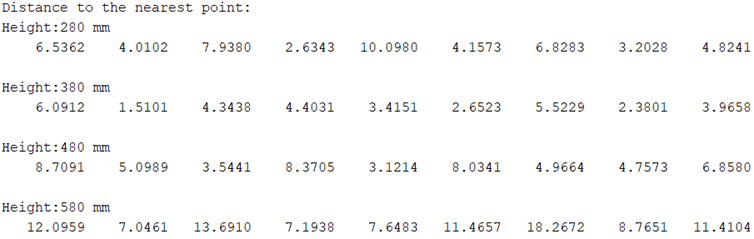
\includegraphics[width=0.65\linewidth]{Image/Code-Display/matlab_280.png}
    \caption[The detection result while index=1000000 and H=280]
    {\centering \textbf{The detection result while index=1000000 and H=280.}}
    \label{fig:matlab_280}
\end{figure}
\begin{figure}[H] %[H] "corresponds to start the figure Here" 
    \centering %alignment can be flushleft or flushright
    \captionsetup{labelsep=colon}
    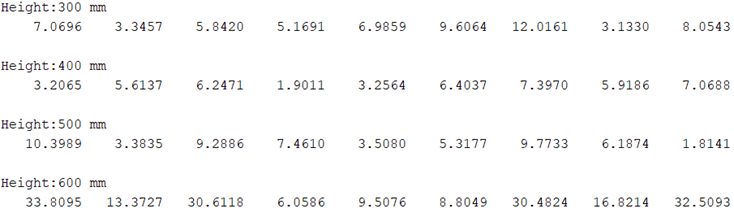
\includegraphics[width=0.65\linewidth]{Image/Code-Display/matlab_300.png}
    \caption[The detection result while index=1000000 and H=300]
    {\centering \textbf{The detection result while index=1000000 and H=300.}}
    \label{fig:matlab_300}
\end{figure}

% change to new page
\newpage